\documentclass[1p]{elsarticle_modified}
%\bibliographystyle{elsarticle-num}

%\usepackage[colorlinks]{hyperref}
%\usepackage{abbrmath_seonhwa} %\Abb, \Ascr, \Acal ,\Abf, \Afrak
\usepackage{amsfonts}
\usepackage{amssymb}
\usepackage{amsmath}
\usepackage{amsthm}
\usepackage{scalefnt}
\usepackage{amsbsy}
\usepackage{kotex}
\usepackage{caption}
\usepackage{subfig}
\usepackage{color}
\usepackage{graphicx}
\usepackage{xcolor} %% white, black, red, green, blue, cyan, magenta, yellow
\usepackage{float}
\usepackage{setspace}
\usepackage{hyperref}

\usepackage{tikz}
\usetikzlibrary{arrows}

\usepackage{multirow}
\usepackage{array} % fixed length table
\usepackage{hhline}

%%%%%%%%%%%%%%%%%%%%%
\makeatletter
\renewcommand*\env@matrix[1][\arraystretch]{%
	\edef\arraystretch{#1}%
	\hskip -\arraycolsep
	\let\@ifnextchar\new@ifnextchar
	\array{*\c@MaxMatrixCols c}}
\makeatother %https://tex.stackexchange.com/questions/14071/how-can-i-increase-the-line-spacing-in-a-matrix
%%%%%%%%%%%%%%%

\usepackage[normalem]{ulem}

\newcommand{\msout}[1]{\ifmmode\text{\sout{\ensuremath{#1}}}\else\sout{#1}\fi}
%SOURCE: \msout is \stkout macro in https://tex.stackexchange.com/questions/20609/strikeout-in-math-mode

\newcommand{\cancel}[1]{
	\ifmmode
	{\color{red}\msout{#1}}
	\else
	{\color{red}\sout{#1}}
	\fi
}

\newcommand{\add}[1]{
	{\color{blue}\uwave{#1}}
}

\newcommand{\replace}[2]{
	\ifmmode
	{\color{red}\msout{#1}}{\color{blue}\uwave{#2}}
	\else
	{\color{red}\sout{#1}}{\color{blue}\uwave{#2}}
	\fi
}

\newcommand{\Sol}{\mathcal{S}} %segment
\newcommand{\D}{D} %diagram
\newcommand{\A}{\mathcal{A}} %arc


%%%%%%%%%%%%%%%%%%%%%%%%%%%%%5 test

\def\sl{\operatorname{\textup{SL}}(2,\Cbb)}
\def\psl{\operatorname{\textup{PSL}}(2,\Cbb)}
\def\quan{\mkern 1mu \triangleright \mkern 1mu}

\theoremstyle{definition}
\newtheorem{thm}{Theorem}[section]
\newtheorem{prop}[thm]{Proposition}
\newtheorem{lem}[thm]{Lemma}
\newtheorem{ques}[thm]{Question}
\newtheorem{cor}[thm]{Corollary}
\newtheorem{defn}[thm]{Definition}
\newtheorem{exam}[thm]{Example}
\newtheorem{rmk}[thm]{Remark}
\newtheorem{alg}[thm]{Algorithm}

\newcommand{\I}{\sqrt{-1}}
\begin{document}

%\begin{frontmatter}
%
%\title{Boundary parabolic representations of knots up to 8 crossings}
%
%%% Group authors per affiliation:
%\author{Yunhi Cho} 
%\address{Department of Mathematics, University of Seoul, Seoul, Korea}
%\ead{yhcho@uos.ac.kr}
%
%
%\author{Seonhwa Kim} %\fnref{s_kim}}
%\address{Center for Geometry and Physics, Institute for Basic Science, Pohang, 37673, Korea}
%\ead{ryeona17@ibs.re.kr}
%
%\author{Hyuk Kim}
%\address{Department of Mathematical Sciences, Seoul National University, Seoul 08826, Korea}
%\ead{hyukkim@snu.ac.kr}
%
%\author{Seokbeom Yoon}
%\address{Department of Mathematical Sciences, Seoul National University, Seoul, 08826,  Korea}
%\ead{sbyoon15@snu.ac.kr}
%
%\begin{abstract}
%We find all boundary parabolic representation of knots up to 8 crossings.
%
%\end{abstract}
%\begin{keyword}
%    \MSC[2010] 57M25 
%\end{keyword}
%
%\end{frontmatter}

%\linenumbers
%\tableofcontents
%
\newcommand\colored[1]{\textcolor{white}{\rule[-0.35ex]{0.8em}{1.4ex}}\kern-0.8em\color{red} #1}%
%\newcommand\colored[1]{\textcolor{white}{ #1}\kern-2.17ex	\textcolor{white}{ #1}\kern-1.81ex	\textcolor{white}{ #1}\kern-2.15ex\color{red}#1	}

{\Large $\underline{12a_{0194}~(K12a_{0194})}$}

\setlength{\tabcolsep}{10pt}
\renewcommand{\arraystretch}{1.6}
\vspace{1cm}\begin{tabular}{m{100pt}>{\centering\arraybackslash}m{274pt}}
\multirow{5}{120pt}{
	\centering
	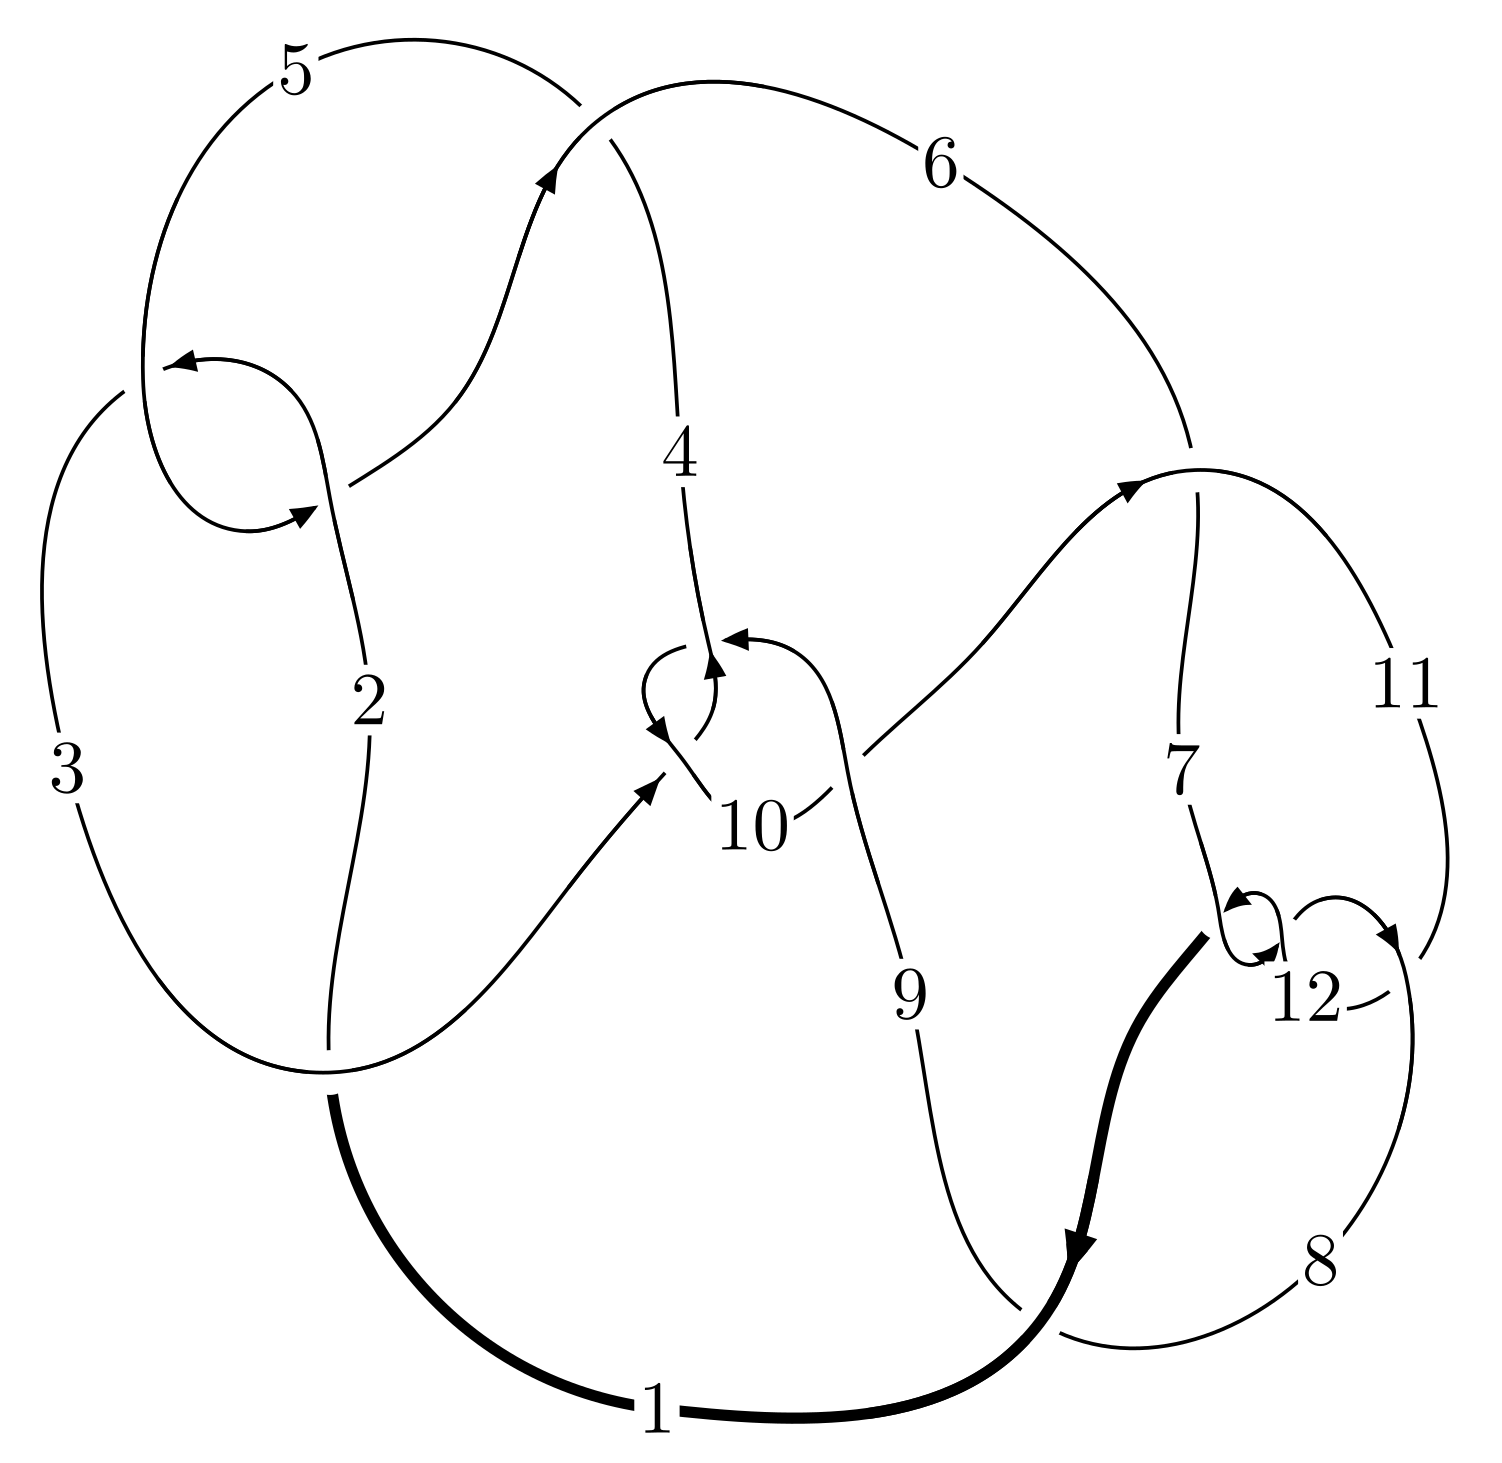
\includegraphics[width=112pt]{../../../GIT/diagram.site/Diagrams/png/995_12a_0194.png}\\
\ \ \ A knot diagram\footnotemark}&
\allowdisplaybreaks
\textbf{Linearized knot diagam} \\
\cline{2-2}
 &
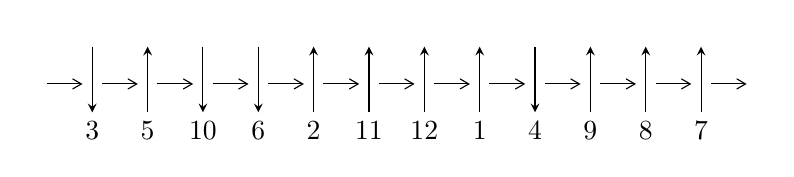
\begin{tikzpicture}[x=20pt, y=17pt]
	% nodes
	\node (C0) at (0, 0) {};
	\node (C1) at (1, 0) {};
	\node (C1U) at (1, +1) {};
	\node (C1D) at (1, -1) {3};

	\node (C2) at (2, 0) {};
	\node (C2U) at (2, +1) {};
	\node (C2D) at (2, -1) {5};

	\node (C3) at (3, 0) {};
	\node (C3U) at (3, +1) {};
	\node (C3D) at (3, -1) {10};

	\node (C4) at (4, 0) {};
	\node (C4U) at (4, +1) {};
	\node (C4D) at (4, -1) {6};

	\node (C5) at (5, 0) {};
	\node (C5U) at (5, +1) {};
	\node (C5D) at (5, -1) {2};

	\node (C6) at (6, 0) {};
	\node (C6U) at (6, +1) {};
	\node (C6D) at (6, -1) {11};

	\node (C7) at (7, 0) {};
	\node (C7U) at (7, +1) {};
	\node (C7D) at (7, -1) {12};

	\node (C8) at (8, 0) {};
	\node (C8U) at (8, +1) {};
	\node (C8D) at (8, -1) {1};

	\node (C9) at (9, 0) {};
	\node (C9U) at (9, +1) {};
	\node (C9D) at (9, -1) {4};

	\node (C10) at (10, 0) {};
	\node (C10U) at (10, +1) {};
	\node (C10D) at (10, -1) {9};

	\node (C11) at (11, 0) {};
	\node (C11U) at (11, +1) {};
	\node (C11D) at (11, -1) {8};

	\node (C12) at (12, 0) {};
	\node (C12U) at (12, +1) {};
	\node (C12D) at (12, -1) {7};
	\node (C13) at (13, 0) {};

	% arrows
	\draw[->,>={angle 60}]
	(C0) edge (C1) (C1) edge (C2) (C2) edge (C3) (C3) edge (C4) (C4) edge (C5) (C5) edge (C6) (C6) edge (C7) (C7) edge (C8) (C8) edge (C9) (C9) edge (C10) (C10) edge (C11) (C11) edge (C12) (C12) edge (C13) ;	\draw[->,>=stealth]
	(C1U) edge (C1D) (C2D) edge (C2U) (C3U) edge (C3D) (C4U) edge (C4D) (C5D) edge (C5U) (C6D) edge (C6U) (C7D) edge (C7U) (C8D) edge (C8U) (C9U) edge (C9D) (C10D) edge (C10U) (C11D) edge (C11U) (C12D) edge (C12U) ;
	\end{tikzpicture} \\
\hhline{~~} \\& 
\textbf{Solving Sequence} \\ \cline{2-2} 
 &
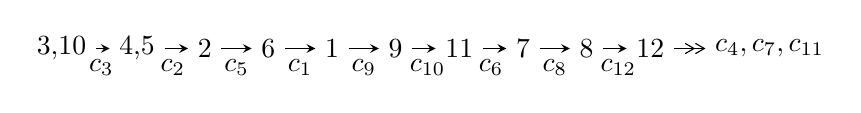
\begin{tikzpicture}[x=23pt, y=7pt]
	% node
	\node (A0) at (-1/8, 0) {3,10};
	\node (A1) at (17/16, 0) {4,5};
	\node (A2) at (17/8, 0) {2};
	\node (A3) at (25/8, 0) {6};
	\node (A4) at (33/8, 0) {1};
	\node (A5) at (41/8, 0) {9};
	\node (A6) at (49/8, 0) {11};
	\node (A7) at (57/8, 0) {7};
	\node (A8) at (65/8, 0) {8};
	\node (A9) at (73/8, 0) {12};
	\node (C1) at (1/2, -1) {$c_{3}$};
	\node (C2) at (13/8, -1) {$c_{2}$};
	\node (C3) at (21/8, -1) {$c_{5}$};
	\node (C4) at (29/8, -1) {$c_{1}$};
	\node (C5) at (37/8, -1) {$c_{9}$};
	\node (C6) at (45/8, -1) {$c_{10}$};
	\node (C7) at (53/8, -1) {$c_{6}$};
	\node (C8) at (61/8, -1) {$c_{8}$};
	\node (C9) at (69/8, -1) {$c_{12}$};
	\node (A10) at (11, 0) {$c_{4},c_{7},c_{11}$};

	% edge
	\draw[->,>=stealth]	
	(A0) edge (A1) (A1) edge (A2) (A2) edge (A3) (A3) edge (A4) (A4) edge (A5) (A5) edge (A6) (A6) edge (A7) (A7) edge (A8) (A8) edge (A9) ;
	\draw[->>,>={angle 60}]	
	(A9) edge (A10);
\end{tikzpicture} \\ 

\end{tabular} \\

\footnotetext{
The image of knot diagram is generated by the software ``\textbf{Draw programme}" developed by Andrew Bartholomew(\url{http://www.layer8.co.uk/maths/draw/index.htm\#Running-draw}), where we modified some parts for our purpose(\url{https://github.com/CATsTAILs/LinksPainter}).
}\phantom \\ \newline 
\centering \textbf{Ideals for irreducible components\footnotemark of $X_{\text{par}}$} 
 
\begin{align*}
I^u_{1}&=\langle 
-1.93196\times10^{140} u^{86}+6.66096\times10^{139} u^{85}+\cdots+1.09402\times10^{141} b+3.74745\times10^{141},\\
\phantom{I^u_{1}}&\phantom{= \langle  }1.59602\times10^{141} u^{86}-1.20857\times10^{140} u^{85}+\cdots+2.18804\times10^{141} a-3.03570\times10^{142},\;u^{87}- u^{86}+\cdots-32 u-64\rangle \\
\\
I^v_{1}&=\langle 
a,\;v^4+v^3+v^2+b+v+1,\;v^6+v^5+v^4+2 v^3+v^2+1\rangle \\
\end{align*}
\raggedright * 2 irreducible components of $\dim_{\mathbb{C}}=0$, with total 93 representations.\\
\footnotetext{All coefficients of polynomials are rational numbers. But the coefficients are sometimes approximated in decimal forms when there is not enough margin.}
\newpage
\renewcommand{\arraystretch}{1}
\centering \section*{I. $I^u_{1}= \langle -1.93\times10^{140} u^{86}+6.66\times10^{139} u^{85}+\cdots+1.09\times10^{141} b+3.75\times10^{141},\;1.60\times10^{141} u^{86}-1.21\times10^{140} u^{85}+\cdots+2.19\times10^{141} a-3.04\times10^{142},\;u^{87}- u^{86}+\cdots-32 u-64 \rangle$}
\flushleft \textbf{(i) Arc colorings}\\
\begin{tabular}{m{7pt} m{180pt} m{7pt} m{180pt} }
\flushright $a_{3}=$&$\begin{pmatrix}1\\0\end{pmatrix}$ \\
\flushright $a_{10}=$&$\begin{pmatrix}0\\u\end{pmatrix}$ \\
\flushright $a_{4}=$&$\begin{pmatrix}1\\u^2\end{pmatrix}$ \\
\flushright $a_{5}=$&$\begin{pmatrix}-0.729429 u^{86}+0.0552353 u^{85}+\cdots+62.6495 u+13.8741\\0.176593 u^{86}-0.0608853 u^{85}+\cdots-15.4584 u-3.42540\end{pmatrix}$ \\
\flushright $a_{2}=$&$\begin{pmatrix}0.0681336 u^{86}-0.709362 u^{85}+\cdots+54.5898 u+49.3534\\-0.134816 u^{86}+0.459791 u^{85}+\cdots-32.0043 u-32.4889\end{pmatrix}$ \\
\flushright $a_{6}=$&$\begin{pmatrix}0.0681336 u^{86}-0.709362 u^{85}+\cdots+54.5898 u+49.3534\\-0.398582 u^{86}+0.178985 u^{85}+\cdots+15.8456 u-8.54975\end{pmatrix}$ \\
\flushright $a_{1}=$&$\begin{pmatrix}-0.0666825 u^{86}-0.249571 u^{85}+\cdots+22.5855 u+16.8646\\-0.134816 u^{86}+0.459791 u^{85}+\cdots-32.0043 u-32.4889\end{pmatrix}$ \\
\flushright $a_{9}=$&$\begin{pmatrix}u\\u^3+u\end{pmatrix}$ \\
\flushright $a_{11}=$&$\begin{pmatrix}u^3\\u^5+u^3+u\end{pmatrix}$ \\
\flushright $a_{7}=$&$\begin{pmatrix}-0.368646 u^{86}-0.527148 u^{85}+\cdots+71.9013 u+40.4381\\-0.312704 u^{86}+0.0963934 u^{85}+\cdots+15.1995 u-3.76857\end{pmatrix}$ \\
\flushright $a_{8}=$&$\begin{pmatrix}-0.439933 u^{86}-0.447080 u^{85}+\cdots+58.1327 u+22.1757\\-0.0174712 u^{86}+0.0259493 u^{85}+\cdots-0.972693 u-3.56818\end{pmatrix}$ \\
\flushright $a_{12}=$&$\begin{pmatrix}0.774940 u^{86}-1.07849 u^{85}+\cdots+41.4842 u+76.3652\\-0.00285224 u^{86}-0.0798040 u^{85}+\cdots+8.17160 u+2.44523\end{pmatrix}$\\&\end{tabular}
\flushleft \textbf{(ii) Obstruction class $= -1$}\\~\\
\flushleft \textbf{(iii) Cusp Shapes $= 0.00629905 u^{86}-0.167117 u^{85}+\cdots+11.7485 u+43.8850$}\\~\\
\newpage\renewcommand{\arraystretch}{1}
\flushleft \textbf{(iv) u-Polynomials at the component}\newline \\
\begin{tabular}{m{50pt}|m{274pt}}
Crossings & \hspace{64pt}u-Polynomials at each crossing \\
\hline $$\begin{aligned}c_{1},c_{4}\end{aligned}$$&$\begin{aligned}
&u^{87}+30 u^{86}+\cdots+10 u-1
\end{aligned}$\\
\hline $$\begin{aligned}c_{2},c_{5}\end{aligned}$$&$\begin{aligned}
&u^{87}+4 u^{86}+\cdots+2 u+1
\end{aligned}$\\
\hline $$\begin{aligned}c_{3},c_{9}\end{aligned}$$&$\begin{aligned}
&u^{87}- u^{86}+\cdots-32 u-64
\end{aligned}$\\
\hline $$\begin{aligned}c_{6},c_{8}\end{aligned}$$&$\begin{aligned}
&u^{87}-3 u^{86}+\cdots+313 u-73
\end{aligned}$\\
\hline $$\begin{aligned}c_{7},c_{11},c_{12}\end{aligned}$$&$\begin{aligned}
&u^{87}+3 u^{86}+\cdots- u-1
\end{aligned}$\\
\hline $$\begin{aligned}c_{10}\end{aligned}$$&$\begin{aligned}
&u^{87}-35 u^{86}+\cdots-44032 u+4096
\end{aligned}$\\
\hline
\end{tabular}\\~\\
\newpage\renewcommand{\arraystretch}{1}
\flushleft \textbf{(v) Riley Polynomials at the component}\newline \\
\begin{tabular}{m{50pt}|m{274pt}}
Crossings & \hspace{64pt}Riley Polynomials at each crossing \\
\hline $$\begin{aligned}c_{1},c_{4}\end{aligned}$$&$\begin{aligned}
&y^{87}+58 y^{86}+\cdots+94 y-1
\end{aligned}$\\
\hline $$\begin{aligned}c_{2},c_{5}\end{aligned}$$&$\begin{aligned}
&y^{87}+30 y^{86}+\cdots+10 y-1
\end{aligned}$\\
\hline $$\begin{aligned}c_{3},c_{9}\end{aligned}$$&$\begin{aligned}
&y^{87}+35 y^{86}+\cdots-44032 y-4096
\end{aligned}$\\
\hline $$\begin{aligned}c_{6},c_{8}\end{aligned}$$&$\begin{aligned}
&y^{87}-51 y^{86}+\cdots-128331 y-5329
\end{aligned}$\\
\hline $$\begin{aligned}c_{7},c_{11},c_{12}\end{aligned}$$&$\begin{aligned}
&y^{87}+73 y^{86}+\cdots-19 y-1
\end{aligned}$\\
\hline $$\begin{aligned}c_{10}\end{aligned}$$&$\begin{aligned}
&y^{87}+23 y^{86}+\cdots-99614720 y-16777216
\end{aligned}$\\
\hline
\end{tabular}\\~\\
\newpage\flushleft \textbf{(vi) Complex Volumes and Cusp Shapes}
$$\begin{array}{c|c|c}  
\text{Solutions to }I^u_{1}& \I (\text{vol} + \sqrt{-1}CS) & \text{Cusp shape}\\
 \hline 
\begin{aligned}
u &= \phantom{-}0.611285 + 0.788569 I \\
a &= \phantom{-}0.917741 + 0.861333 I \\
b &= -0.082818 + 1.004170 I\end{aligned}
 & -3.36212 - 2.35337 I & \phantom{-0.000000 } 0 \\ \hline\begin{aligned}
u &= \phantom{-}0.611285 - 0.788569 I \\
a &= \phantom{-}0.917741 - 0.861333 I \\
b &= -0.082818 - 1.004170 I\end{aligned}
 & -3.36212 + 2.35337 I & \phantom{-0.000000 } 0 \\ \hline\begin{aligned}
u &= \phantom{-}0.443560 + 0.899987 I \\
a &= \phantom{-}0.644315 - 0.499952 I \\
b &= -0.526359 - 1.058500 I\end{aligned}
 & -2.47271 - 2.75618 I & \phantom{-0.000000 } 0 \\ \hline\begin{aligned}
u &= \phantom{-}0.443560 - 0.899987 I \\
a &= \phantom{-}0.644315 + 0.499952 I \\
b &= -0.526359 + 1.058500 I\end{aligned}
 & -2.47271 + 2.75618 I & \phantom{-0.000000 } 0 \\ \hline\begin{aligned}
u &= \phantom{-}0.767266 + 0.648567 I \\
a &= \phantom{-}1.04401 + 1.12977 I \\
b &= \phantom{-}0.055082 + 1.005560 I\end{aligned}
 & -6.09885 + 4.42777 I & \phantom{-0.000000 } 0 \\ \hline\begin{aligned}
u &= \phantom{-}0.767266 - 0.648567 I \\
a &= \phantom{-}1.04401 - 1.12977 I \\
b &= \phantom{-}0.055082 - 1.005560 I\end{aligned}
 & -6.09885 - 4.42777 I & \phantom{-0.000000 } 0 \\ \hline\begin{aligned}
u &= \phantom{-}0.277378 + 0.974111 I \\
a &= -1.10874 - 1.67118 I \\
b &= \phantom{-}0.716351 + 0.750458 I\end{aligned}
 & \phantom{-}3.27239 + 1.34065 I & \phantom{-0.000000 } 0 \\ \hline\begin{aligned}
u &= \phantom{-}0.277378 - 0.974111 I \\
a &= -1.10874 + 1.67118 I \\
b &= \phantom{-}0.716351 - 0.750458 I\end{aligned}
 & \phantom{-}3.27239 - 1.34065 I & \phantom{-0.000000 } 0 \\ \hline\begin{aligned}
u &= \phantom{-}0.678907 + 0.702812 I \\
a &= \phantom{-}0.769386 + 0.217668 I \\
b &= -0.650762 + 0.511807 I\end{aligned}
 & -4.66548 - 1.46210 I & \phantom{-0.000000 -}0. + 3.02931 I \\ \hline\begin{aligned}
u &= \phantom{-}0.678907 - 0.702812 I \\
a &= \phantom{-}0.769386 - 0.217668 I \\
b &= -0.650762 - 0.511807 I\end{aligned}
 & -4.66548 + 1.46210 I & \phantom{-0.000000 } 0. - 3.02931 I\\
 \hline 
 \end{array}$$\newpage$$\begin{array}{c|c|c}  
\text{Solutions to }I^u_{1}& \I (\text{vol} + \sqrt{-1}CS) & \text{Cusp shape}\\
 \hline 
\begin{aligned}
u &= -0.768238 + 0.688700 I \\
a &= \phantom{-}0.634804 + 0.441462 I \\
b &= -0.618764 + 1.016630 I\end{aligned}
 & -6.05440 - 3.49870 I & \phantom{-0.000000 } 0 \\ \hline\begin{aligned}
u &= -0.768238 - 0.688700 I \\
a &= \phantom{-}0.634804 - 0.441462 I \\
b &= -0.618764 - 1.016630 I\end{aligned}
 & -6.05440 + 3.49870 I & \phantom{-0.000000 } 0 \\ \hline\begin{aligned}
u &= -1.008650 + 0.241433 I \\
a &= \phantom{-}0.684736 - 0.311760 I \\
b &= -0.725433 - 0.765619 I\end{aligned}
 & \phantom{-}0.50208 + 3.44185 I & \phantom{-0.000000 } 0 \\ \hline\begin{aligned}
u &= -1.008650 - 0.241433 I \\
a &= \phantom{-}0.684736 + 0.311760 I \\
b &= -0.725433 + 0.765619 I\end{aligned}
 & \phantom{-}0.50208 - 3.44185 I & \phantom{-0.000000 } 0 \\ \hline\begin{aligned}
u &= \phantom{-}0.426093 + 0.859319 I \\
a &= -3.15793 - 0.28000 I \\
b &= \phantom{-}0.652013 - 0.953417 I\end{aligned}
 & -2.63778 - 0.82623 I & \phantom{-}4.00000 + 3.60231 I \\ \hline\begin{aligned}
u &= \phantom{-}0.426093 - 0.859319 I \\
a &= -3.15793 + 0.28000 I \\
b &= \phantom{-}0.652013 + 0.953417 I\end{aligned}
 & -2.63778 + 0.82623 I & \phantom{-}4.00000 - 3.60231 I \\ \hline\begin{aligned}
u &= -0.695363 + 0.644567 I \\
a &= \phantom{-}1.10625 - 1.01304 I \\
b &= \phantom{-}0.026957 - 0.964064 I\end{aligned}
 & -1.31652 - 0.83169 I & \phantom{-}1.65300 + 1.09851 I \\ \hline\begin{aligned}
u &= -0.695363 - 0.644567 I \\
a &= \phantom{-}1.10625 + 1.01304 I \\
b &= \phantom{-}0.026957 + 0.964064 I\end{aligned}
 & -1.31652 + 0.83169 I & \phantom{-}1.65300 - 1.09851 I \\ \hline\begin{aligned}
u &= \phantom{-}0.520735 + 0.931628 I \\
a &= \phantom{-}0.792847 + 0.788022 I \\
b &= -0.164125 + 1.058190 I\end{aligned}
 & -3.08368 - 2.00968 I & \phantom{-0.000000 } 0 \\ \hline\begin{aligned}
u &= \phantom{-}0.520735 - 0.931628 I \\
a &= \phantom{-}0.792847 - 0.788022 I \\
b &= -0.164125 - 1.058190 I\end{aligned}
 & -3.08368 + 2.00968 I & \phantom{-0.000000 } 0\\
 \hline 
 \end{array}$$\newpage$$\begin{array}{c|c|c}  
\text{Solutions to }I^u_{1}& \I (\text{vol} + \sqrt{-1}CS) & \text{Cusp shape}\\
 \hline 
\begin{aligned}
u &= \phantom{-}1.005790 + 0.366180 I \\
a &= \phantom{-}0.691862 + 0.291804 I \\
b &= -0.735938 + 0.721753 I\end{aligned}
 & \phantom{-}3.86176 + 0.42107 I & \phantom{-0.000000 } 0 \\ \hline\begin{aligned}
u &= \phantom{-}1.005790 - 0.366180 I \\
a &= \phantom{-}0.691862 - 0.291804 I \\
b &= -0.735938 - 0.721753 I\end{aligned}
 & \phantom{-}3.86176 - 0.42107 I & \phantom{-0.000000 } 0 \\ \hline\begin{aligned}
u &= \phantom{-}1.006180 + 0.368157 I \\
a &= \phantom{-}0.639735 - 0.387808 I \\
b &= -0.692514 - 0.944335 I\end{aligned}
 & -0.04609 + 1.98521 I & \phantom{-0.000000 } 0 \\ \hline\begin{aligned}
u &= \phantom{-}1.006180 - 0.368157 I \\
a &= \phantom{-}0.639735 + 0.387808 I \\
b &= -0.692514 + 0.944335 I\end{aligned}
 & -0.04609 - 1.98521 I & \phantom{-0.000000 } 0 \\ \hline\begin{aligned}
u &= -0.421885 + 0.985583 I \\
a &= -2.66540 + 0.10722 I \\
b &= \phantom{-}0.684806 + 0.957414 I\end{aligned}
 & \phantom{-}2.63586 + 4.03889 I & \phantom{-0.000000 } 0 \\ \hline\begin{aligned}
u &= -0.421885 - 0.985583 I \\
a &= -2.66540 - 0.10722 I \\
b &= \phantom{-}0.684806 - 0.957414 I\end{aligned}
 & \phantom{-}2.63586 - 4.03889 I & \phantom{-0.000000 } 0 \\ \hline\begin{aligned}
u &= -0.296732 + 1.041850 I \\
a &= \phantom{-}0.777629 - 0.073278 I \\
b &= -0.689752 - 0.183697 I\end{aligned}
 & \phantom{-}0.964622 - 0.562642 I & \phantom{-0.000000 } 0 \\ \hline\begin{aligned}
u &= -0.296732 - 1.041850 I \\
a &= \phantom{-}0.777629 + 0.073278 I \\
b &= -0.689752 + 0.183697 I\end{aligned}
 & \phantom{-}0.964622 + 0.562642 I & \phantom{-0.000000 } 0 \\ \hline\begin{aligned}
u &= -0.331769 + 0.849752 I \\
a &= \phantom{-}0.664057 + 0.509027 I \\
b &= -0.498045 + 1.039790 I\end{aligned}
 & \phantom{-}1.93817 - 0.98719 I & \phantom{-}8.58368 - 0.93595 I \\ \hline\begin{aligned}
u &= -0.331769 - 0.849752 I \\
a &= \phantom{-}0.664057 - 0.509027 I \\
b &= -0.498045 - 1.039790 I\end{aligned}
 & \phantom{-}1.93817 + 0.98719 I & \phantom{-}8.58368 + 0.93595 I\\
 \hline 
 \end{array}$$\newpage$$\begin{array}{c|c|c}  
\text{Solutions to }I^u_{1}& \I (\text{vol} + \sqrt{-1}CS) & \text{Cusp shape}\\
 \hline 
\begin{aligned}
u &= -1.019790 + 0.453057 I \\
a &= \phantom{-}0.692708 - 0.276370 I \\
b &= -0.751523 - 0.691973 I\end{aligned}
 & -0.55415 - 4.35219 I & \phantom{-0.000000 } 0 \\ \hline\begin{aligned}
u &= -1.019790 - 0.453057 I \\
a &= \phantom{-}0.692708 + 0.276370 I \\
b &= -0.751523 + 0.691973 I\end{aligned}
 & -0.55415 + 4.35219 I & \phantom{-0.000000 } 0 \\ \hline\begin{aligned}
u &= \phantom{-}0.594895 + 0.947229 I \\
a &= -0.324433 - 1.258840 I \\
b &= \phantom{-}0.746602 + 0.626637 I\end{aligned}
 & -3.92192 - 3.46935 I & \phantom{-0.000000 } 0 \\ \hline\begin{aligned}
u &= \phantom{-}0.594895 - 0.947229 I \\
a &= -0.324433 + 1.258840 I \\
b &= \phantom{-}0.746602 - 0.626637 I\end{aligned}
 & -3.92192 + 3.46935 I & \phantom{-0.000000 } 0 \\ \hline\begin{aligned}
u &= \phantom{-}0.149465 + 0.867093 I \\
a &= \phantom{-}0.686866 - 0.538383 I \\
b &= -0.444261 - 1.034670 I\end{aligned}
 & -1.54609 + 4.58317 I & \phantom{-}5.10158 - 4.29853 I \\ \hline\begin{aligned}
u &= \phantom{-}0.149465 - 0.867093 I \\
a &= \phantom{-}0.686866 + 0.538383 I \\
b &= -0.444261 + 1.034670 I\end{aligned}
 & -1.54609 - 4.58317 I & \phantom{-}5.10158 + 4.29853 I \\ \hline\begin{aligned}
u &= \phantom{-}0.411198 + 1.044420 I \\
a &= \phantom{-}0.765130 + 0.098490 I \\
b &= -0.714320 + 0.248220 I\end{aligned}
 & \phantom{-}4.23995 - 3.36961 I & \phantom{-0.000000 } 0 \\ \hline\begin{aligned}
u &= \phantom{-}0.411198 - 1.044420 I \\
a &= \phantom{-}0.765130 - 0.098490 I \\
b &= -0.714320 - 0.248220 I\end{aligned}
 & \phantom{-}4.23995 + 3.36961 I & \phantom{-0.000000 } 0 \\ \hline\begin{aligned}
u &= -0.740949 + 0.850608 I \\
a &= \phantom{-}0.826055 - 0.975867 I \\
b &= -0.041288 - 1.076880 I\end{aligned}
 & -9.58781 + 2.79623 I & \phantom{-0.000000 } 0 \\ \hline\begin{aligned}
u &= -0.740949 - 0.850608 I \\
a &= \phantom{-}0.826055 + 0.975867 I \\
b &= -0.041288 + 1.076880 I\end{aligned}
 & -9.58781 - 2.79623 I & \phantom{-0.000000 } 0\\
 \hline 
 \end{array}$$\newpage$$\begin{array}{c|c|c}  
\text{Solutions to }I^u_{1}& \I (\text{vol} + \sqrt{-1}CS) & \text{Cusp shape}\\
 \hline 
\begin{aligned}
u &= -0.446275 + 1.037880 I \\
a &= -0.71304 + 1.33524 I \\
b &= \phantom{-}0.757142 - 0.696856 I\end{aligned}
 & \phantom{-}2.32576 + 2.18173 I & \phantom{-0.000000 } 0 \\ \hline\begin{aligned}
u &= -0.446275 - 1.037880 I \\
a &= -0.71304 - 1.33524 I \\
b &= \phantom{-}0.757142 + 0.696856 I\end{aligned}
 & \phantom{-}2.32576 - 2.18173 I & \phantom{-0.000000 } 0 \\ \hline\begin{aligned}
u &= -1.026800 + 0.483421 I \\
a &= \phantom{-}0.628167 + 0.397780 I \\
b &= -0.692708 + 0.975062 I\end{aligned}
 & \phantom{-}3.09256 - 5.88380 I & \phantom{-0.000000 } 0 \\ \hline\begin{aligned}
u &= -1.026800 - 0.483421 I \\
a &= \phantom{-}0.628167 - 0.397780 I \\
b &= -0.692708 - 0.975062 I\end{aligned}
 & \phantom{-}3.09256 + 5.88380 I & \phantom{-0.000000 } 0 \\ \hline\begin{aligned}
u &= -0.233192 + 0.805989 I \\
a &= -1.13555 + 2.48104 I \\
b &= \phantom{-}0.652662 - 0.757523 I\end{aligned}
 & -2.01462 - 4.26726 I & \phantom{-}5.97179 + 2.61130 I \\ \hline\begin{aligned}
u &= -0.233192 - 0.805989 I \\
a &= -1.13555 - 2.48104 I \\
b &= \phantom{-}0.652662 + 0.757523 I\end{aligned}
 & -2.01462 + 4.26726 I & \phantom{-}5.97179 - 2.61130 I \\ \hline\begin{aligned}
u &= -0.488848 + 1.054160 I \\
a &= \phantom{-}0.753394 - 0.112714 I \\
b &= -0.738176 - 0.286575 I\end{aligned}
 & -0.22381 + 7.35518 I & \phantom{-0.000000 } 0 \\ \hline\begin{aligned}
u &= -0.488848 - 1.054160 I \\
a &= \phantom{-}0.753394 + 0.112714 I \\
b &= -0.738176 + 0.286575 I\end{aligned}
 & -0.22381 - 7.35518 I & \phantom{-0.000000 } 0 \\ \hline\begin{aligned}
u &= -0.607515 + 0.995263 I \\
a &= \phantom{-}0.748024 - 0.842364 I \\
b &= -0.136497 - 1.103500 I\end{aligned}
 & -0.23467 + 5.86188 I & \phantom{-0.000000 } 0 \\ \hline\begin{aligned}
u &= -0.607515 - 0.995263 I \\
a &= \phantom{-}0.748024 + 0.842364 I \\
b &= -0.136497 + 1.103500 I\end{aligned}
 & -0.23467 - 5.86188 I & \phantom{-0.000000 } 0\\
 \hline 
 \end{array}$$\newpage$$\begin{array}{c|c|c}  
\text{Solutions to }I^u_{1}& \I (\text{vol} + \sqrt{-1}CS) & \text{Cusp shape}\\
 \hline 
\begin{aligned}
u &= \phantom{-}1.043830 + 0.551455 I \\
a &= \phantom{-}0.620829 - 0.402944 I \\
b &= -0.694009 - 0.993135 I\end{aligned}
 & -1.46195 + 9.86196 I & \phantom{-0.000000 } 0 \\ \hline\begin{aligned}
u &= \phantom{-}1.043830 - 0.551455 I \\
a &= \phantom{-}0.620829 + 0.402944 I \\
b &= -0.694009 + 0.993135 I\end{aligned}
 & -1.46195 - 9.86196 I & \phantom{-0.000000 } 0 \\ \hline\begin{aligned}
u &= \phantom{-}0.540953 + 1.061670 I \\
a &= -2.32849 - 0.37630 I \\
b &= \phantom{-}0.698997 - 0.991276 I\end{aligned}
 & \phantom{-}1.43879 - 7.72271 I & \phantom{-0.000000 } 0 \\ \hline\begin{aligned}
u &= \phantom{-}0.540953 - 1.061670 I \\
a &= -2.32849 + 0.37630 I \\
b &= \phantom{-}0.698997 + 0.991276 I\end{aligned}
 & \phantom{-}1.43879 + 7.72271 I & \phantom{-0.000000 } 0 \\ \hline\begin{aligned}
u &= -0.657070 + 0.997761 I \\
a &= -2.30139 + 0.72609 I \\
b &= \phantom{-}0.677860 + 1.017760 I\end{aligned}
 & -5.07559 + 8.90900 I & \phantom{-0.000000 } 0 \\ \hline\begin{aligned}
u &= -0.657070 - 0.997761 I \\
a &= -2.30139 - 0.72609 I \\
b &= \phantom{-}0.677860 - 1.017760 I\end{aligned}
 & -5.07559 - 8.90900 I & \phantom{-0.000000 } 0 \\ \hline\begin{aligned}
u &= \phantom{-}0.668410 + 0.428154 I \\
a &= \phantom{-}0.670160 - 0.423926 I \\
b &= -0.603421 - 0.947278 I\end{aligned}
 & -0.45864 + 3.05031 I & \phantom{-}0.11561 - 3.71074 I \\ \hline\begin{aligned}
u &= \phantom{-}0.668410 - 0.428154 I \\
a &= \phantom{-}0.670160 + 0.423926 I \\
b &= -0.603421 + 0.947278 I\end{aligned}
 & -0.45864 - 3.05031 I & \phantom{-}0.11561 + 3.71074 I \\ \hline\begin{aligned}
u &= \phantom{-}0.652989 + 1.019560 I \\
a &= \phantom{-}0.726453 + 0.866754 I \\
b &= -0.122757 + 1.123020 I\end{aligned}
 & -4.94082 - 9.82420 I & \phantom{-0.000000 } 0 \\ \hline\begin{aligned}
u &= \phantom{-}0.652989 - 1.019560 I \\
a &= \phantom{-}0.726453 - 0.866754 I \\
b &= -0.122757 - 1.123020 I\end{aligned}
 & -4.94082 + 9.82420 I & \phantom{-0.000000 } 0\\
 \hline 
 \end{array}$$\newpage$$\begin{array}{c|c|c}  
\text{Solutions to }I^u_{1}& \I (\text{vol} + \sqrt{-1}CS) & \text{Cusp shape}\\
 \hline 
\begin{aligned}
u &= \phantom{-}0.527998 + 0.508519 I \\
a &= \phantom{-}1.38834 + 0.49257 I \\
b &= \phantom{-}0.025988 + 0.717177 I\end{aligned}
 & -4.08095 - 1.96025 I & -2.32551 + 3.82515 I \\ \hline\begin{aligned}
u &= \phantom{-}0.527998 - 0.508519 I \\
a &= \phantom{-}1.38834 - 0.49257 I \\
b &= \phantom{-}0.025988 - 0.717177 I\end{aligned}
 & -4.08095 + 1.96025 I & -2.32551 - 3.82515 I \\ \hline\begin{aligned}
u &= -0.250839 + 0.646005 I \\
a &= \phantom{-}0.913229 - 0.095011 I \\
b &= -0.377028 - 0.231372 I\end{aligned}
 & \phantom{-}0.322925 + 0.980399 I & \phantom{-}5.93960 - 6.62047 I \\ \hline\begin{aligned}
u &= -0.250839 - 0.646005 I \\
a &= \phantom{-}0.913229 + 0.095011 I \\
b &= -0.377028 + 0.231372 I\end{aligned}
 & \phantom{-}0.322925 - 0.980399 I & \phantom{-}5.93960 + 6.62047 I \\ \hline\begin{aligned}
u &= -0.561413 + 1.185130 I \\
a &= -0.662931 + 0.987024 I \\
b &= \phantom{-}0.824524 - 0.680211 I\end{aligned}
 & \phantom{-}3.53114 + 2.02176 I & \phantom{-0.000000 } 0 \\ \hline\begin{aligned}
u &= -0.561413 - 1.185130 I \\
a &= -0.662931 - 0.987024 I \\
b &= \phantom{-}0.824524 + 0.680211 I\end{aligned}
 & \phantom{-}3.53114 - 2.02176 I & \phantom{-0.000000 } 0 \\ \hline\begin{aligned}
u &= \phantom{-}0.029916 + 1.327490 I \\
a &= -1.49885 - 0.68928 I \\
b &= \phantom{-}0.804293 + 0.856431 I\end{aligned}
 & \phantom{-}6.54252 - 1.34989 I & \phantom{-0.000000 } 0 \\ \hline\begin{aligned}
u &= \phantom{-}0.029916 - 1.327490 I \\
a &= -1.49885 + 0.68928 I \\
b &= \phantom{-}0.804293 - 0.856431 I\end{aligned}
 & \phantom{-}6.54252 + 1.34989 I & \phantom{-0.000000 } 0 \\ \hline\begin{aligned}
u &= \phantom{-}0.047029 + 1.330660 I \\
a &= -1.59556 + 0.59324 I \\
b &= \phantom{-}0.798778 - 0.877711 I\end{aligned}
 & \phantom{-}10.37450 - 2.98463 I & \phantom{-0.000000 } 0 \\ \hline\begin{aligned}
u &= \phantom{-}0.047029 - 1.330660 I \\
a &= -1.59556 - 0.59324 I \\
b &= \phantom{-}0.798778 + 0.877711 I\end{aligned}
 & \phantom{-}10.37450 + 2.98463 I & \phantom{-0.000000 } 0\\
 \hline 
 \end{array}$$\newpage$$\begin{array}{c|c|c}  
\text{Solutions to }I^u_{1}& \I (\text{vol} + \sqrt{-1}CS) & \text{Cusp shape}\\
 \hline 
\begin{aligned}
u &= -0.121603 + 1.328060 I \\
a &= -1.68238 - 0.49161 I \\
b &= \phantom{-}0.792331 + 0.897528 I\end{aligned}
 & \phantom{-}6.41712 + 7.31572 I & \phantom{-0.000000 } 0 \\ \hline\begin{aligned}
u &= -0.121603 - 1.328060 I \\
a &= -1.68238 + 0.49161 I \\
b &= \phantom{-}0.792331 - 0.897528 I\end{aligned}
 & \phantom{-}6.41712 - 7.31572 I & \phantom{-0.000000 } 0 \\ \hline\begin{aligned}
u &= \phantom{-}0.634374 + 1.173840 I \\
a &= -2.00540 - 0.45132 I \\
b &= \phantom{-}0.722792 - 1.019870 I\end{aligned}
 & \phantom{-}2.49663 - 7.82179 I & \phantom{-0.000000 } 0 \\ \hline\begin{aligned}
u &= \phantom{-}0.634374 - 1.173840 I \\
a &= -2.00540 + 0.45132 I \\
b &= \phantom{-}0.722792 + 1.019870 I\end{aligned}
 & \phantom{-}2.49663 + 7.82179 I & \phantom{-0.000000 } 0 \\ \hline\begin{aligned}
u &= \phantom{-}0.633489 + 1.184630 I \\
a &= -0.577053 - 0.930602 I \\
b &= \phantom{-}0.836929 + 0.657205 I\end{aligned}
 & \phantom{-}6.44169 - 6.28675 I & \phantom{-0.000000 } 0 \\ \hline\begin{aligned}
u &= \phantom{-}0.633489 - 1.184630 I \\
a &= -0.577053 + 0.930602 I \\
b &= \phantom{-}0.836929 - 0.657205 I\end{aligned}
 & \phantom{-}6.44169 + 6.28675 I & \phantom{-0.000000 } 0 \\ \hline\begin{aligned}
u &= -0.622610 + 0.177262 I \\
a &= \phantom{-}0.884623 + 0.156178 I \\
b &= \phantom{-}0.346087 - 0.160520 I\end{aligned}
 & -2.55006 - 3.29913 I & \phantom{-}1.11145 + 2.49429 I \\ \hline\begin{aligned}
u &= -0.622610 - 0.177262 I \\
a &= \phantom{-}0.884623 - 0.156178 I \\
b &= \phantom{-}0.346087 + 0.160520 I\end{aligned}
 & -2.55006 + 3.29913 I & \phantom{-}1.11145 - 2.49429 I \\ \hline\begin{aligned}
u &= -0.679060 + 1.174990 I \\
a &= -0.522511 + 0.901931 I \\
b &= \phantom{-}0.842463 - 0.641024 I\end{aligned}
 & \phantom{-}1.73423 + 10.47340 I & \phantom{-0.000000 } 0 \\ \hline\begin{aligned}
u &= -0.679060 - 1.174990 I \\
a &= -0.522511 - 0.901931 I \\
b &= \phantom{-}0.842463 + 0.641024 I\end{aligned}
 & \phantom{-}1.73423 - 10.47340 I & \phantom{-0.000000 } 0\\
 \hline 
 \end{array}$$\newpage$$\begin{array}{c|c|c}  
\text{Solutions to }I^u_{1}& \I (\text{vol} + \sqrt{-1}CS) & \text{Cusp shape}\\
 \hline 
\begin{aligned}
u &= -0.696216 + 1.175180 I \\
a &= -1.94109 + 0.54914 I \\
b &= \phantom{-}0.720267 + 1.035200 I\end{aligned}
 & \phantom{-}5.29166 + 12.11040 I & \phantom{-0.000000 } 0 \\ \hline\begin{aligned}
u &= -0.696216 - 1.175180 I \\
a &= -1.94109 - 0.54914 I \\
b &= \phantom{-}0.720267 - 1.035200 I\end{aligned}
 & \phantom{-}5.29166 - 12.11040 I & \phantom{-0.000000 } 0 \\ \hline\begin{aligned}
u &= \phantom{-}0.733904 + 1.165900 I \\
a &= -1.91300 - 0.61390 I \\
b &= \phantom{-}0.716303 - 1.044050 I\end{aligned}
 & \phantom{-}0.5090 - 16.2964 I & \phantom{-0.000000 } 0 \\ \hline\begin{aligned}
u &= \phantom{-}0.733904 - 1.165900 I \\
a &= -1.91300 + 0.61390 I \\
b &= \phantom{-}0.716303 + 1.044050 I\end{aligned}
 & \phantom{-}0.5090 + 16.2964 I & \phantom{-0.000000 } 0 \\ \hline\begin{aligned}
u &= -0.509418 + 0.232441 I \\
a &= \phantom{-}0.763520 - 0.371468 I \\
b &= -0.541403 - 0.775770 I\end{aligned}
 & \phantom{-}0.16334 + 1.55638 I & -0.76791 - 2.56835 I \\ \hline\begin{aligned}
u &= -0.509418 - 0.232441 I \\
a &= \phantom{-}0.763520 + 0.371468 I \\
b &= -0.541403 + 0.775770 I\end{aligned}
 & \phantom{-}0.16334 - 1.55638 I & -0.76791 + 2.56835 I \\ \hline\begin{aligned}
u &= \phantom{-}0.557201\phantom{ +0.000000I} \\
a &= \phantom{-}0.897719\phantom{ +0.000000I} \\
b &= \phantom{-}0.285348\phantom{ +0.000000I}\end{aligned}
 & \phantom{-}1.51878\phantom{ +0.000000I} & \phantom{-}6.53030\phantom{ +0.000000I}\\
 \hline 
 \end{array}$$\newpage\newpage\renewcommand{\arraystretch}{1}
\centering \section*{II. $I^v_{1}= \langle a,\;v^4+v^3+v^2+b+v+1,\;v^6+v^5+v^4+2 v^3+v^2+1 \rangle$}
\flushleft \textbf{(i) Arc colorings}\\
\begin{tabular}{m{7pt} m{180pt} m{7pt} m{180pt} }
\flushright $a_{3}=$&$\begin{pmatrix}1\\0\end{pmatrix}$ \\
\flushright $a_{10}=$&$\begin{pmatrix}v\\0\end{pmatrix}$ \\
\flushright $a_{4}=$&$\begin{pmatrix}1\\0\end{pmatrix}$ \\
\flushright $a_{5}=$&$\begin{pmatrix}0\\- v^4- v^3- v^2- v-1\end{pmatrix}$ \\
\flushright $a_{2}=$&$\begin{pmatrix}1\\v^4+v^3+v^2+v\end{pmatrix}$ \\
\flushright $a_{6}=$&$\begin{pmatrix}- v^4- v^3- v^2- v-1\\- v^4- v^3- v^2- v\end{pmatrix}$ \\
\flushright $a_{1}=$&$\begin{pmatrix}v^4+v^3+v^2+v+1\\v^4+v^3+v^2+v\end{pmatrix}$ \\
\flushright $a_{9}=$&$\begin{pmatrix}v\\0\end{pmatrix}$ \\
\flushright $a_{11}=$&$\begin{pmatrix}v\\0\end{pmatrix}$ \\
\flushright $a_{7}=$&$\begin{pmatrix}- v^4- v\\- v^4- v^3- v^2- v\end{pmatrix}$ \\
\flushright $a_{8}=$&$\begin{pmatrix}0\\- v^5- v^4- v^3- v^2- v\end{pmatrix}$ \\
\flushright $a_{12}=$&$\begin{pmatrix}v\\v^4+v^3+v\end{pmatrix}$\\&\end{tabular}
\flushleft \textbf{(ii) Obstruction class $= 1$}\\~\\
\flushleft \textbf{(iii) Cusp Shapes $= -4 v^5-9 v^4-9 v^3-8 v^2-6 v+1$}\\~\\
\newpage\renewcommand{\arraystretch}{1}
\flushleft \textbf{(iv) u-Polynomials at the component}\newline \\
\begin{tabular}{m{50pt}|m{274pt}}
Crossings & \hspace{64pt}u-Polynomials at each crossing \\
\hline $$\begin{aligned}c_{1},c_{4},c_{5}\end{aligned}$$&$\begin{aligned}
&(u^2- u+1)^3
\end{aligned}$\\
\hline $$\begin{aligned}c_{2}\end{aligned}$$&$\begin{aligned}
&(u^2+u+1)^3
\end{aligned}$\\
\hline $$\begin{aligned}c_{3},c_{9},c_{10}\end{aligned}$$&$\begin{aligned}
&u^6
\end{aligned}$\\
\hline $$\begin{aligned}c_{6},c_{8}\end{aligned}$$&$\begin{aligned}
&(u^3- u^2+1)^2
\end{aligned}$\\
\hline $$\begin{aligned}c_{7}\end{aligned}$$&$\begin{aligned}
&(u^3+u^2+2 u+1)^2
\end{aligned}$\\
\hline $$\begin{aligned}c_{11},c_{12}\end{aligned}$$&$\begin{aligned}
&(u^3- u^2+2 u-1)^2
\end{aligned}$\\
\hline
\end{tabular}\\~\\
\newpage\renewcommand{\arraystretch}{1}
\flushleft \textbf{(v) Riley Polynomials at the component}\newline \\
\begin{tabular}{m{50pt}|m{274pt}}
Crossings & \hspace{64pt}Riley Polynomials at each crossing \\
\hline $$\begin{aligned}c_{1},c_{2},c_{4}\\c_{5}\end{aligned}$$&$\begin{aligned}
&(y^2+y+1)^3
\end{aligned}$\\
\hline $$\begin{aligned}c_{3},c_{9},c_{10}\end{aligned}$$&$\begin{aligned}
&y^6
\end{aligned}$\\
\hline $$\begin{aligned}c_{6},c_{8}\end{aligned}$$&$\begin{aligned}
&(y^3- y^2+2 y-1)^2
\end{aligned}$\\
\hline $$\begin{aligned}c_{7},c_{11},c_{12}\end{aligned}$$&$\begin{aligned}
&(y^3+3 y^2+2 y-1)^2
\end{aligned}$\\
\hline
\end{tabular}\\~\\
\newpage\flushleft \textbf{(vi) Complex Volumes and Cusp Shapes}
$$\begin{array}{c|c|c}  
\text{Solutions to }I^v_{1}& \I (\text{vol} + \sqrt{-1}CS) & \text{Cusp shape}\\
 \hline 
\begin{aligned}
v &= \phantom{-}0.206350 + 1.132320 I \\
a &= \phantom{-0.000000 } 0 \\
b &= -0.500000 + 0.866025 I\end{aligned}
 & -3.02413 - 4.85801 I & -1.45566 + 6.64456 I \\ \hline\begin{aligned}
v &= \phantom{-}0.206350 - 1.132320 I \\
a &= \phantom{-0.000000 } 0 \\
b &= -0.500000 - 0.866025 I\end{aligned}
 & -3.02413 + 4.85801 I & -1.45566 - 6.64456 I \\ \hline\begin{aligned}
v &= -1.083790 + 0.387453 I \\
a &= \phantom{-0.000000 } 0 \\
b &= -0.500000 + 0.866025 I\end{aligned}
 & -3.02413 + 0.79824 I & \phantom{-}2.09851 + 0.12339 I \\ \hline\begin{aligned}
v &= -1.083790 - 0.387453 I \\
a &= \phantom{-0.000000 } 0 \\
b &= -0.500000 - 0.866025 I\end{aligned}
 & -3.02413 - 0.79824 I & \phantom{-}2.09851 - 0.12339 I \\ \hline\begin{aligned}
v &= \phantom{-}0.377439 + 0.653743 I \\
a &= \phantom{-0.000000 } 0 \\
b &= -0.500000 - 0.866025 I\end{aligned}
 & \phantom{-}1.11345 + 2.02988 I & \phantom{-}5.85715 - 4.49037 I \\ \hline\begin{aligned}
v &= \phantom{-}0.377439 - 0.653743 I \\
a &= \phantom{-0.000000 } 0 \\
b &= -0.500000 + 0.866025 I\end{aligned}
 & \phantom{-}1.11345 - 2.02988 I & \phantom{-}5.85715 + 4.49037 I\\
 \hline 
 \end{array}$$\newpage
\newpage\renewcommand{\arraystretch}{1}
\centering \section*{ III. u-Polynomials}
\begin{tabular}{m{50pt}|m{274pt}}
Crossings & \hspace{64pt}u-Polynomials at each crossing \\
\hline $$\begin{aligned}c_{1},c_{4}\end{aligned}$$&$\begin{aligned}
&((u^2- u+1)^3)(u^{87}+30 u^{86}+\cdots+10 u-1)
\end{aligned}$\\
\hline $$\begin{aligned}c_{2}\end{aligned}$$&$\begin{aligned}
&((u^2+u+1)^3)(u^{87}+4 u^{86}+\cdots+2 u+1)
\end{aligned}$\\
\hline $$\begin{aligned}c_{3},c_{9}\end{aligned}$$&$\begin{aligned}
&u^6(u^{87}- u^{86}+\cdots-32 u-64)
\end{aligned}$\\
\hline $$\begin{aligned}c_{5}\end{aligned}$$&$\begin{aligned}
&((u^2- u+1)^3)(u^{87}+4 u^{86}+\cdots+2 u+1)
\end{aligned}$\\
\hline $$\begin{aligned}c_{6},c_{8}\end{aligned}$$&$\begin{aligned}
&((u^3- u^2+1)^2)(u^{87}-3 u^{86}+\cdots+313 u-73)
\end{aligned}$\\
\hline $$\begin{aligned}c_{7}\end{aligned}$$&$\begin{aligned}
&((u^3+u^2+2 u+1)^2)(u^{87}+3 u^{86}+\cdots- u-1)
\end{aligned}$\\
\hline $$\begin{aligned}c_{10}\end{aligned}$$&$\begin{aligned}
&u^6(u^{87}-35 u^{86}+\cdots-44032 u+4096)
\end{aligned}$\\
\hline $$\begin{aligned}c_{11},c_{12}\end{aligned}$$&$\begin{aligned}
&((u^3- u^2+2 u-1)^2)(u^{87}+3 u^{86}+\cdots- u-1)
\end{aligned}$\\
\hline
\end{tabular}\newpage\renewcommand{\arraystretch}{1}
\centering \section*{ IV. Riley Polynomials}
\begin{tabular}{m{50pt}|m{274pt}}
Crossings & \hspace{64pt}Riley Polynomials at each crossing \\
\hline $$\begin{aligned}c_{1},c_{4}\end{aligned}$$&$\begin{aligned}
&((y^2+y+1)^3)(y^{87}+58 y^{86}+\cdots+94 y-1)
\end{aligned}$\\
\hline $$\begin{aligned}c_{2},c_{5}\end{aligned}$$&$\begin{aligned}
&((y^2+y+1)^3)(y^{87}+30 y^{86}+\cdots+10 y-1)
\end{aligned}$\\
\hline $$\begin{aligned}c_{3},c_{9}\end{aligned}$$&$\begin{aligned}
&y^6(y^{87}+35 y^{86}+\cdots-44032 y-4096)
\end{aligned}$\\
\hline $$\begin{aligned}c_{6},c_{8}\end{aligned}$$&$\begin{aligned}
&((y^3- y^2+2 y-1)^2)(y^{87}-51 y^{86}+\cdots-128331 y-5329)
\end{aligned}$\\
\hline $$\begin{aligned}c_{7},c_{11},c_{12}\end{aligned}$$&$\begin{aligned}
&((y^3+3 y^2+2 y-1)^2)(y^{87}+73 y^{86}+\cdots-19 y-1)
\end{aligned}$\\
\hline $$\begin{aligned}c_{10}\end{aligned}$$&$\begin{aligned}
&y^6(y^{87}+23 y^{86}+\cdots-9.96147\times10^{7} y-1.67772\times10^{7})
\end{aligned}$\\
\hline
\end{tabular}
\vskip 2pc
\end{document}